% !TEX root = ../main.tex
\chapter{一些重要的\LaTeX{}环境}\label{chap:evm}

本模版中的公式、插图、表格和章节等,均用\texttt{$\backslash$lable\{<key>\}}来在\LaTeX{}代码中标记位置,用\texttt{$\backslash$ref\{<key>\}}来在代码中引用,其中\texttt{<key>}为自定义的标签。

\section{公式示例}

文中的公式建议使用\texttt{amsmath}宏包的\texttt{align}环境,该环境在对多行公式对齐方面具有很大的优势,具体的讨论请看知乎用户\href{https://www.zhihu.com/people/bo-xue-duo-wen-63}{\strong{博闻多学}}的\href{https://www.zhihu.com/question/477805692/answer/2045084752}{\strong{回答}}。

下面进行公式示例。普通公式:
\begin{align}
    a+b=x.
\end{align}
带有积分和分隔的公式:
\begin{align}
   \int^{\infty}_{0} f(x)\dd{x}, \qquad \oint_{C} f(z)\dd {z}.
\end{align}
多行公式:
\begin{align}
    \left(1+x\right)^{\alpha} &= \sum^{\infty}_{n=0}\left(\begin{matrix} \alpha \\ n\end{matrix}\right)x^n \nonumber \\ 
    &= 1 + \alpha x + \frac{\alpha(\alpha-1)}{2!}x^2 + \cdots + \frac{\alpha(\alpha-1)\cdots(\alpha-n+1)}{n!} + \cdots
    \label{eqn:taylorseries}
\end{align}
这里注意,对不需要编号的行要取消公式编号,即要在该行公式的源代码后边使用\texttt{$\backslash$nonumber}命令。

公式的引用示例:\ref{eqn:taylorseries}为泰勒级数。

\section{插图示例}

文中插图的插图建议使用\texttt{graphicx}宏包的\texttt{figure}环境搭配\texttt{$\backslash$includegraphics}命令。例如:
\begin{figure}[!htp]
	\centering
	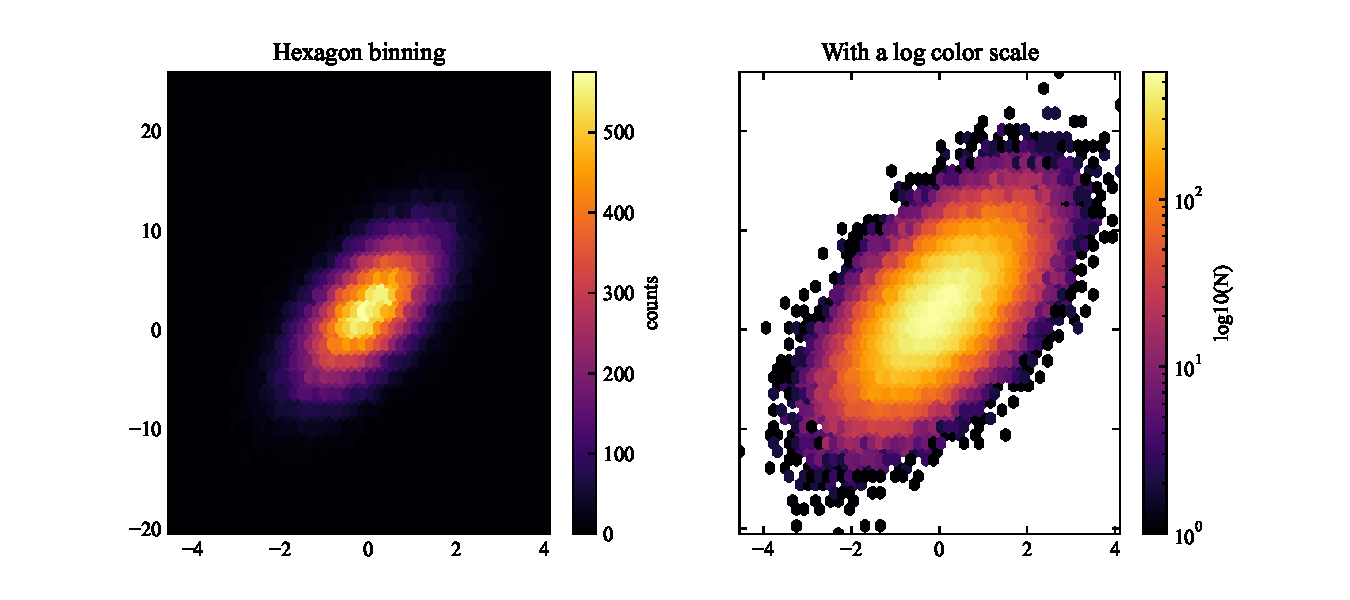
\includegraphics[width=1\textwidth]{figures/hexbin.pdf}
	\caption{六边形分bin图}
	\label{fig:hexbin}
\end{figure}
\begin{figure}[!htp]
	\centering
    \begin{subfigure}{0.45\textwidth}
        \centering
	    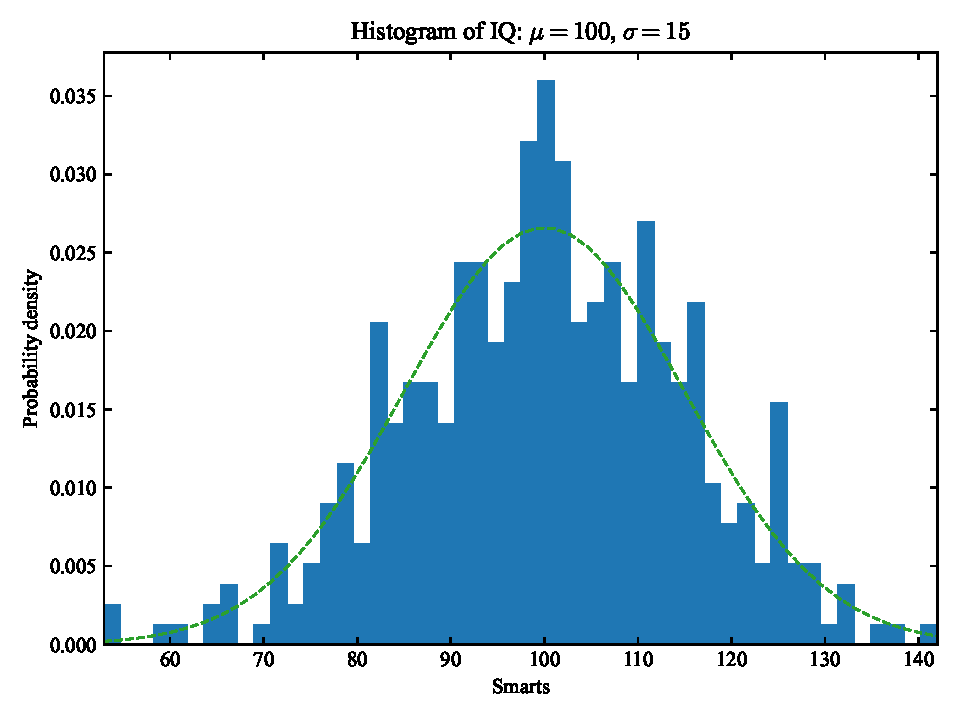
\includegraphics[width=1\textwidth]{figures/histogram.pdf}
	    \caption{柱状图}
    \end{subfigure}
    \begin{subfigure}{0.45\textwidth}
        \centering
	    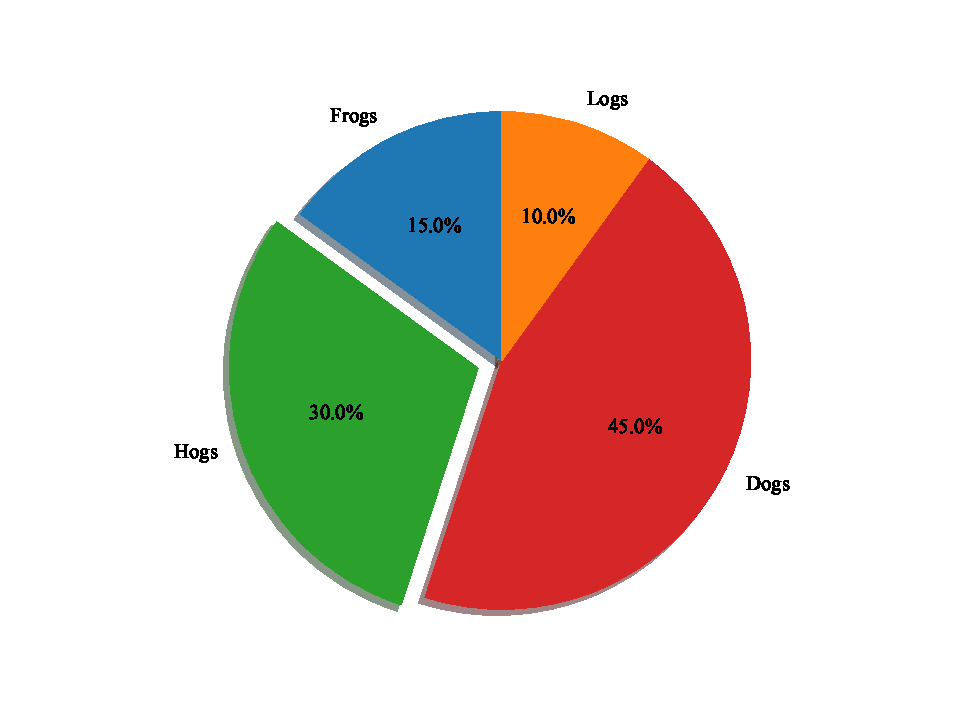
\includegraphics[width=1\textwidth]{figures/piechart.pdf}
	    \caption{饼状图}
    \end{subfigure}
    \caption{子图示例}
    \label{fig:subfig}
\end{figure}

插图的引用示例:\ref{fig:hexbin}是普通插图。

\section{表格示例}

文中的表格建议使用\texttt{table}环境里嵌套\texttt{tabular}环境,简单的表格样式一般采用三线表。
\begin{table}[!htp]
    \caption{2022年北京冬奥会奖牌榜}
    \label{tab:01}
    \centering
    \begin{tabular}{ccrrrr}
        \hline
        总排名 & 国家/地区 & 金牌 & 银牌 & 铜牌 & 合计  \\ 
        \hline
        1 & 挪威 & 16 & 8 & 13 & 37\\
        2 & 德国 & 12 & 10 & 5 & 27\\
        3 & 中国 & 9 & 4 & 2 & 15\\
        4 & 美国 & 8 & 10 & 7 & 25\\
        5 & 瑞典 & 8 & 5 & 5 & 18\\
        6 & 荷兰 & 8 & 5 & 4 & 17\\
        7 & 奥地利 & 7 & 7 & 4 & 18\\
        8 & 法国 & 7 & 2 & 5 & 14\\
        9 & 俄罗斯奥林匹克委员会\tablefootnote{俄罗斯由于被禁赛,不能以国家名义参加奥运会,不能使用国旗和国歌。因此俄罗斯代表团绕过禁令,以俄罗斯奥委会(Russian Olympic Committee)的名义参赛,以俄罗斯奥委会的会旗作为代表团的团旗,以柴可夫斯基的《第一钢琴协奏曲》作为团歌\cite{ROC}。} 
            & 6 & 12 & 14 & 32\\ 
        10 & 法国 & 5 & 7 & 2 & 14\\
        \hline
    \end{tabular}
\end{table}
这里需要注意,如果需要在表格内添加注释,请使用\texttt{tablefootnote}宏包的\texttt{$\backslash$tablefootnote}命令。如果要制作长表格,请使用\texttt{longtable}宏包的\texttt{longtable}环境。

表格的引用示例:\ref{tab:01}是2022年北京冬奥会奖牌榜。

\section{其他数学环境示例}

以下是本模版预设的数学环境示例:

\begin{assumption}[连续统假设]
    不存在一个基数绝对大于可数集而绝对小于实数集的集合。
\end{assumption}
\begin{axiom}[平行公理]
    若两条直线都与第三条直线相交,并且在同一边的内角之和小于两个直角,则这两条直线在这一边必定相交。
\end{axiom}
\begin{conjecture}[黎曼猜想]
    黎曼$\zeta$函数
    \begin{align}
        \zeta(s) = \frac{1}{1^s} + \frac{1}{2^s} + \frac{1}{3^s} + \frac{1}{4^s} + \cdots
    \end{align}
    非平凡点的实数部分是$\frac{1}{2}$。
\end{conjecture}
\begin{definition}[定义的定义]
    对一个概念或者词或者词组的定义是描写其内涵,即描写其所有和仅有的元素的共有特征。其外延是所有这个概念、词或者词组包含的事物。
\end{definition}
\begin{example}
    举个栗子。
\end{example}
\begin{exercise}
    TiMi,发出学习的声音。
\end{exercise}
\begin{lemma}[欧几里得引理]
    如果一个正整数整除另外两个正整数的乘积,第一个整数与第二个整数互质,那么第一个整数整除第三个整数。
\end{lemma}
\begin{problem}
    花儿为什么这样红?
\end{problem}
\begin{proposition}
    通过一个不在直线上的点,有且仅有一条不与该直线相交的直线。
\end{proposition}
\begin{theorem}[诺特定理]
    对于每个局部作用下的可微对称性,存在一个对应的守恒流。另言之,每个连续对称性都有着相应的守恒定律。
\end{theorem}
\begin{corollary}
    推论往往在定理后出现。如果命题B能够被简单明了的从命题A推导出,则称B为A的推论。
\end{corollary}
\begin{solution}
    这个问题无解。
\end{solution}
\begin{proof}
    因为爱情,不会轻易悲伤,所以一切都是幸福的模样。
\end{proof}

\section{代码示例}

在论文中插入代码,我们使用的是\texttt{listings}宏包的\texttt{lstlisting}环境,如:
\begin{lstlisting}[language=python]
import numpy as np
import matplotlib.pyplot as plt

# Fixing random state for reproducibility
np.random.seed(19680801)

dt = 0.01
t = np.arange(0, 30, dt)
nse1 = np.random.randn(len(t))                 # white noise 1
nse2 = np.random.randn(len(t))                 # white noise 2
    
# Two signals with a coherent part at 10Hz and a random part
s1 = np.sin(2 * np.pi * 10 * t) + nse1
s2 = np.sin(2 * np.pi * 10 * t) + nse2

fig, axs = plt.subplots(2, 1)
axs[0].plot(t, s1, t, s2)
axs[0].set_xlim(0, 2)
axs[0].set_xlabel('time')
axs[0].set_ylabel('s1 and s2')
axs[0].grid(True)
 
cxy, f = axs[1].cohere(s1, s2, 256, 1. / dt)
axs[1].set_ylabel('coherence')

fig.tight_layout()
plt.show()
\end{lstlisting}
或\texttt{$\backslash$lstinputlisting}命令,如:
\lstinputlisting[language=Python]{codes/cohere.py}
建议代码不设置\texttt{caption}选项,也不要使用\texttt{$\backslash$ref}来引用,因为我没给代码环境设置中文标签 (> <)。

\section{参考文献}\label{sec:bibstyle}

\subsection{引用格式}

\begin{enumerate}
    \item 参考文献为论文中所有引文、引用观点以及对论文有重要影响和启发的文献;
    \item 参考文献按在论文中出现的先后依次排序;个别学科若通用该学科惯用的排序规范,可以例外;
    \item 参考文献内容一般排列在论文末尾 (论文篇幅较大且引用文献较多的,可在每章末尾注出),序码与论文加注处对应;
    \item 参考文献标注格式:
        \begin{enumerate}
            \item 期刊:[序号] 作者. 文章题目. 刊名, 出版年份, 卷号(期号): 页码
            \item 图书:[序号] 著者. 书名. 版次(2版以上). 出版地, 出版年份. 页码
            \item 研讨会论文:[序号] 作者. 文章题目. 会议名称. 地名. 国名. 月份. 年份. 卷号
            \item 学位论文:[序号] 作者. 论文题目. 博/硕士论文. 校名. 页码、
            \item 电子文献:[序号] 主要责任者. 电子文献题名. 电子文献的出处或可获得地址, 发表或更新日期/引用日期(任选)
        \end{enumerate}

    例如:
        \begin{enumerate}
            \item 这是一个期刊的引用\cite{LIGOScientific:2017zic};
            \item 这是一个图书的引用\cite{Rubakov:2017xzr};
            \item 这是一个研讨会论文的引用\cite{Tanikawa:2021+x};
            \item 这是博士论文的引用\cite{Migenda:2019xbm,HuangGuoYuan:2020},这是硕论文的引用\cite{Shojaeifar:2015csv,SongRen:2020};
            \item 这是电子文献的引用\cite{Piro:2021oaa,bilibili:read}。
        \end{enumerate}
\end{enumerate}

\subsection{参考文献引用说明}

参考文献的引用格式已经由\texttt{sysuthesis.bst}设置好了。引用时,请将引用信息编入\texttt{ref}文件夹的\texttt{refs.bib}文件中,语法要符合\hologo{BibTeX}格式,并在文中引用处使用\texttt{$\backslash$cite}命令。建议只使用\ref{tab:entrytypes}中的几种\hologo{BibTeX}条目类型(Entry Types)。
\begin{table}[!htp]
    \caption{本模版设置好的\hologo{BibTeX}字段类型}
    \label{tab:entrytypes}
    \centering
    \begin{tabular}{ll}
    \hline
    引用文献的类型 & Entry Types \\
    \hline
    期刊    & \texttt{article} \\
    图书    & \texttt{book} \\
    研讨会论文    & \texttt{conference} \\  
    博士论文    & \texttt{phdthesis} \\
    硕士论文    & \texttt{mastersthesis} \\
    电子文献   & \texttt{online} \\
    \hline
    \end{tabular}
\end{table}
请注意:\strong{如果引用的是中文文献,请再额外添加\texttt{language} 字段,并让它不为空,否者将输出英文引用格式}。例如,这是一个\texttt{article}条目类型的源代码:
\begin{lstlisting}
@article{ZhaoWen:2017twxjz,
    author={赵文 and 张星 and 刘小金 and 张杨 and 王运永 and 张帆 and 肇宇航 and 郭越凡 and 陈奕康 and 艾舜柯 and 朱宗宏 and WANG Xiao-ge and LEBIGOT Eric and 都志辉 and 曹军威 and 钱进 and 殷聪 and 王建波 and BLAIR David and JU Li and ZHAO Chun-nong and WEN Lin-qing},
    title={ 引力波与引力波源 },
    journal={天文学进展},
    language={中文},
    year={2017},
    volume={35},
    number={3},
    pages={316-344},
    month={1},
}
\end{lstlisting}
请点击\cite{ZhaoWen:2017twxjz}查看该期刊文章的引用效果。这是中文图书的引用效果\cite{Huang:2012hxwl}。

\section{注释}
注释:可以用“脚注”或“文后注”来标注引用著作中的一些观点和案例,但全文标注方式应统一,本文统一使用“脚注”\footnote{这里是注释内容。}。
